\section{Medições em laboratório}

No laboratório, montamos o circuito para realizar medições e analisar suas respostas a diversas frequências de sinal de entrada. Essa abordagem abrangente fornece informações práticas sobre o comportamento, estabilidade e desempenho do circuito em diferentes cenários operacionais, permitindo uma comparação posterior com as previsões teóricas.

\begin{figure}[H]
    \centering
    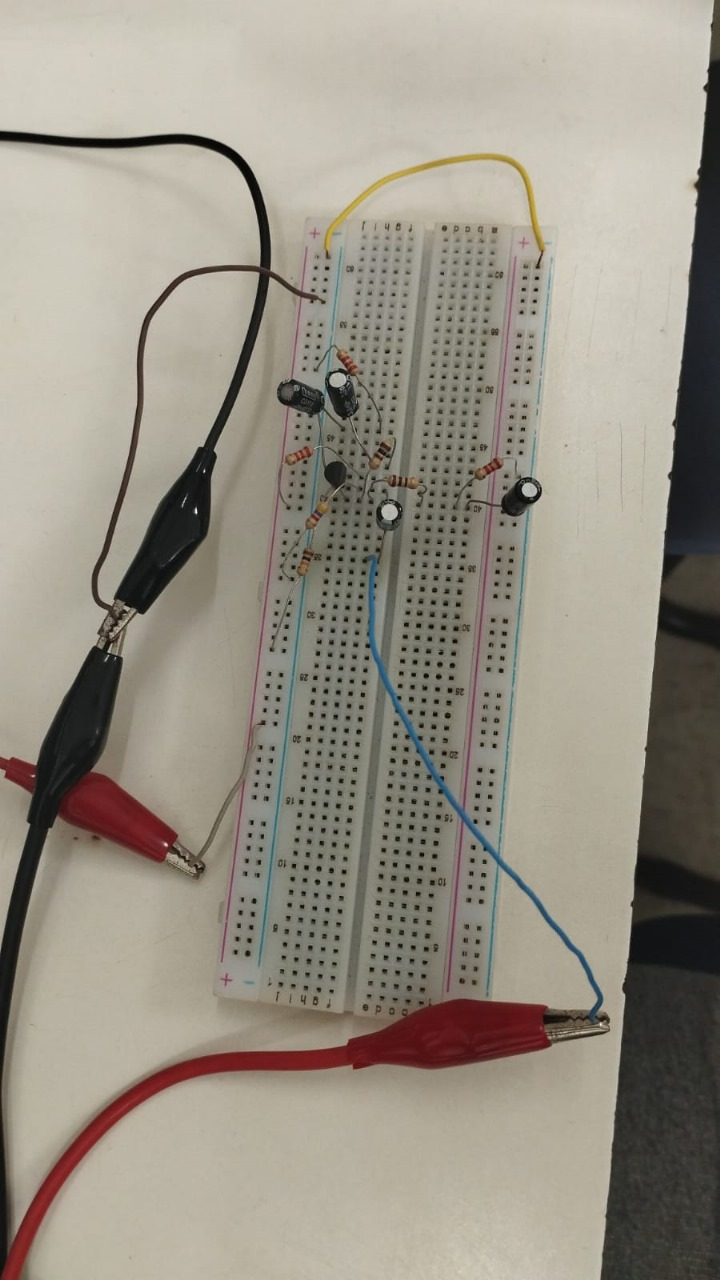
\includegraphics[width=0.5\columnwidth]{Images/circuito_real.jpeg}
    \caption{Circuito montado em laboratório.}
\end{figure}

\subsection{Tabela de componentes}

\begin{figure}[H]
    \centering
    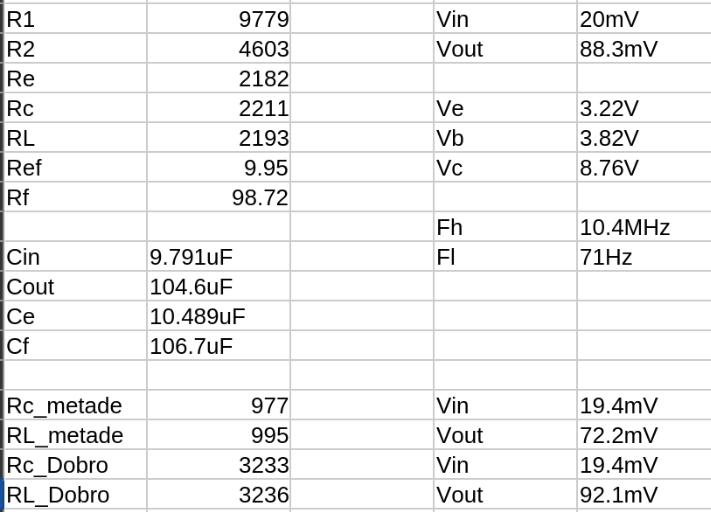
\includegraphics[width=0.5\columnwidth]{Images/componentes_reais.png}
    \caption{Valores dos componentes medidos em laboratório.}
\end{figure}

\subsection{Medidas sob diferentes condições}

Infelizmente, não encontramos as imagens do osciloscópio para as medidas feitas em laboratório no momento de confecção do relatório. Porém, os dados obtidos foram preservados e estão disponíveis abaixo.

\subsubsection{$A_f$ e $F_c$}

Mede-se as amplitudes máximas do sinal de entrada e do sinal de saída e divide-se uma pelo outra. Assim:

\begin{equation}
    \begin{aligned}
         & A_f = \frac{V_{out}}{V_{in}} = \frac{88.3mV}{20mV} = 4.415 \\
         & F_L = 71 Hz                                                \\
         & F_H = 10.3 MHz
    \end{aligned}
\end{equation}

Nota-se que a frequência de corte alta não é confiável devido à precisão dos instrumentos utilizados. Em frequências muito altas, a capacitância do osciloscópio e da protoboard afetam significativamente o comportamento do circuito.

\subsubsection{$A_f$ e $F_c$ alterando $R_c$ e $R_L$}

Nesta medição, reduzem-se na metade os valores de $R_C$ e $R_L$ e averigua-se o ganho do circuito

\begin{equation}
    \begin{aligned}
         & A_{f-50} = \frac{V_{out}}{V_{in}} = \frac{72.2mV}{19.4mV} = 3.72 \\
    \end{aligned}
\end{equation}

Agora dobra-se os valores de $R_C$ e $R_L$ e averigua-se o ganho do circuito

\begin{equation}
    \begin{aligned}
         & A_{f+50} = \frac{V_{out}}{V_{in}} = \frac{92.1mV}{19.4mV} = 4.75 \\
    \end{aligned}
\end{equation}
